\documentclass[a4paper, 20pt,fleqn]{article}
\usepackage[utf8]{inputenc}
\usepackage{jeffe,handout}
\usepackage{eqarrays}
\usepackage{tikz}
\usetikzlibrary{arrows,shapes.gates.logic.US,shapes.gates.logic.IEC,calc}
\usepackage{hyperref}
\usepackage{aurical}
\usepackage[T1]{fontenc}
\usepackage{multirow}

\def\lnot{\mathop{\sim}}
\def\implies{\mathop{\rightarrow}}
\def\xor{\mathop{\oplus}}
\def\andnot{\mathbin{\textit{AndNot}}}
\def\sequence#1#2{\dsequence{#1}{1}{#2}}
\def\dsequence#1#2#3{#1_{#2}, \ldots, #1_{#3}}
\def\ith{$i^{\textrm\scriptsize th}$}

\definecolor{solnblue}{rgb}{0,0,1}
\newenvironment{soln}{\color{solnblue}}{}

\begin{document}
\headers{CPSC 121}{ }{Summer, 2019}

\begin{center}
    \LARGE
    \textbf{HW 4}
    \\[1ex]
    \Large Due: 23:00, Wednesday June 12, 2019  \\
\end{center}
    \LARGE
\begin{tabular}{rl}
 & \\
CS ID 1: &  d6a2b\\
 & \\
CS ID 2: & b9i2b\\
 & \\
\end{tabular}
\large

\noindent\textbf{\LARGE Instructions:}
\begin{enumerate}
\item Do not change the problem statements we are giving you. Simply add your solutions by editing this latex document. To make it easier for the TAs to find your solutions, please use the \textbf{soln} environment we provided as follows:
\begin{soln}
\begin{verbatim}
    \begin{soln}
    My solution is here.
    \end{soln}
\end{verbatim}
\end{soln}
Your solution will then appear in blue, and be easier to differentiate from the questions.
\item Include formatting to clearly distinguish your solutions from the given problem text. Improperly or insufficiently typeset submissions will receive a penalty.
\item If you need more space, add a page between the existing pages using the \texttt{\textbackslash newpage} command.
\item Export the completed assignment as a PDF file for upload to Gradescope.
\item On Gradescope, upload only \textbf{one} copy per partnership. (Instructions for uploading to Gradescope are posted on the assignments page of the course website.)
\item During submission, for each question, please link ALL pages on which your solution appears. Submissions with several linking errors will incur a small penalty.
\item Late submissions will be accepted up to 24 hours past the deadline with a penalty of 20\% of the assignment’s maximum value
\end{enumerate}

\noindent\textbf{\LARGE Academic Conduct:} 
I certify that my assignment follows the academic conduct rules for of CPSC 121 as outlined on the course website. As part of those rules, when collaborating with anyone outside my group, (1) I and my collaborators took no record but names away, and (2) after a suitable break, my group created the assignment I am submitting without help from anyone other than the course staff. \\

\textbf{Version history:}
\begin{itemize}
    \item 2019-05-29 13:22 -- Due date updated
    \item 2019-05-29 02:47 -- Initial version for release
\end{itemize}

\newpage
\normalsize

\begin{question}{1.}[10]


\def\StartsWith#1#2{\textit{Starts}({#1},{#2})}

\item[9] Consider the following sets and predicates: 
  \begin{itemize}
  \item $D$: video game developers
  \item $G$: video game titles
  \item $P$: hardware platforms
  \item $M(d, g)$: developer $d$ made game $g$.
  \item $R(g, p)$: game $g$ released on platform $p$.
  \item $B(d, g)$: developer $d$ bribed a journalist to write a favourable review for game $g$.
  \end{itemize}

  Rewrite each of  the following statements using \textbf{only}  the quantifiers $\forall$
  and $\exists$, the predicates $M$, $R$ and $B$, the domains $D$, $G$, $P$, and $\mathbb{R}$ (the set of real numbers),
  logical connectives, and the operators $=$, $\neq$. $<$, $\le$, $\ge$ and $>$.
  
  If you feel a  sentence is ambiguous, then state your assumed interpretation.
  \begin{question}{a.}[2]

  \item[3] Every developer made a game that released on every platform.
   
   \vspace{2.0in}
   
  \item[3] Some developer bribed a journalist to write a favourable review for a game made by a different developer.
  
  \vspace{2.0in}
   
  \item[3] Some developer bribed journalists to write favourable reviews for every game that the developer made.
  
  \vspace{2.0in}

  \end{question}


\noindent {\em Each of the  next four questions asks you to prove a  theorem. When the theorem
is stated  in English,  it would be  an excellent  idea to first  rewrite it  in predicate
logic, and then  think about the proof  techniques we discussed in class,  and the general
``structure'' of direct or indirect proofs for certain types of statements.}

\item[10] Later in the semester we will discover strategies for proving that for integers $a$, $b$, $c$, $d$, and $m$, if $a\equiv b\bmod{m}$ and $c\equiv d\bmod{m}$, then $a\cdot c\equiv b\cdot d\bmod{m}$, and $a+c\equiv b+d\bmod{m}$. In this problem, we will  investigate the meaning of these statements, and see their implications for number representation. Feel free to use a calculator for parts (a), (b), (f), (g), (h), (i) and (l).

\begin{question}{a.}[0.5]
    \item[0.5] Write the 16-bit unsigned representations of 30924.
    \begin{Questions}
    \vfill
    \end{Questions}
    \item[0.5] What is $30924\bmod 32$, expressed in decimal?
    \begin{Questions}
    \vfill
    \end{Questions}
    \item[0.5] Write the 5-bit unsigned representation of your answer to part (b).
    \begin{Questions}
    \vfill
    \end{Questions}
    \item[0.5] Describe the relationship between your answers to parts (a) and (c).
    \begin{Questions}
    \vfill
    \end{Questions}
    \item[1] Explain how you can compute the remainder when 30924 is divided by 16 (in decimal) \emph{in 10 seconds or less}.
    \begin{Questions}
    \vfill\vfill\eject
    \end{Questions}
    \item[0.5] If $a = 30924$, and $b= 48701$, find the least significant 5 bits of $a+b$ (in binary).
    \begin{Questions}
    \vfill
    \end{Questions}
    \item[0.5] Find $30924 \cdot 8\bmod{32}$ (in decimal).
    \begin{Questions}
    \vfill
    \end{Questions}
    \item[1]
    Write the 16-bit two's complement {\em signed} representation of $-30924$.
    \begin{Questions}
    \vfill
    \end{Questions}
    \item[1]
    Find $-30924\mod{32}$ (in binary).
    \begin{Questions}
    \vfill
    \end{Questions}
    \item[1]
    Describe the relationship between your answers to parts (c) and (i).
    \begin{Questions}
    \vfill\vfill
    \end{Questions}
    \item[0.5] If $a = -30924$, and $b= 16653$, find the least significant 5 bits of $a+b$ (in binary).
    \begin{Questions}
    \vfill
    \end{Questions}
    \item[0.5] Find $-30924 \cdot 8\mod{32}$ (in decimal).
    \begin{Questions}
    \vfill\eject
    \end{Questions}
    \item[2]
    By exploration, we have illustrated some of the implications of the simple rules of modular arithmetic. Show that the rule cannot be extended to the division operation, by finding a {\em counter example}. That is, find unsigned integers $a$, $b$, $c$, $d$, and $m$, so that $a\equiv b\mod{m}$ and $c\equiv d\mod{m}$, but $a/c\not\equiv b/d\mod{m}$.
    \begin{Questions}
    \vfill
    \end{Questions}
    
\end{question}
\vfill\eject


\item[17] Logical Arguments
\begin{question}{a.}[5]

\item[4] Consider the following argument:
\begin{quote}
If there is a chance of rain, or he ate bean chili for lunch, Geoff will not ride his bicycle. Unless Geoff washed his car in the morning, there is no chance of rain. Today Geoff neither washed his car nor ate bean chili. Therefore, Geoff will ride his bicycle today.
\end{quote}

First represent this argument symbolically. Then determine whether it is valid or not.
Justify your answer.
\begin{Questions}
\vfill\eject
\end{Questions}

\item[4] Consider the following argument:
\begin{quote}
If Geoff works hard enough and does not get fired, then he will get paid. If he gets paid, then he will buy food to eat. Geoff has not bought food to eat. Therefore either Geoff did not work hard enough, or he got fired.
\end{quote}

First represent this argument symbolically. Then determine whether it is valid or not.
Justify your answer.
\begin{Questions}
\vfill\eject
\end{Questions}

\item [5]
Consider the following argument:
\begin{quote}
If 30,000 cookies disappeared from Christie's factory, then either Christie destroyed the cookies, or Keebler stole the cookies. If it is not the case that a tree-dwelling elf became the new CEO of Christie and the new Christie CEO colluded with Keebler, then 30,000 cookies disappeared from Christie's factory. If the new Christie CEO did not have a secret meeting with Keebler's industrial spies, then Keebler did not steal the cookies. Christie did not destroy the cookies, and the new Christie CEO had a secret meeting with Keebler's spies. Therefore, Christie's new CEO did not collude with Keebler! No collusion!
\end{quote}

First represent this argument symbolically. Then determine whether it is valid or not.
Justify your answer.
\begin{Questions}
\vfill\eject
\end{Questions}

\item[4]
Determine whether the following argument is valid. If it is valid, show a formal proof and if it is invalid provide a counter-example, i.e. an assignment of truth values that demonstrate a contradiction.


This argument is \underline{~~~~~~~~~~~~~~~~~~~~~}. (Fill in the blank with ``valid'' or ``invalid''.)
\vspace{0.2in}

\hspace{0.4in}\begin{tabular}{r}

$\lnot p \land q$\\
$r \rightarrow p$\\
$\lnot r \rightarrow (s \land t)$\\
$s \rightarrow (t \lor p)$\\
\hline
$\therefore  t  $\\
\end{tabular}
\vspace{0.2in}

Proof:

\hspace{0.4in}\begin{tabular}{r|l}
~~~~~~inference~~~~~~ & rule \\
\hline
 & ~~~~~~~~~~~~~~~~~~~~~~~\\
\hline
 & ~~~~~~~~~~~~~~~~~~~~~~~\\
\hline
 & ~~~~~~~~~~~~~~~~~~~~~~~\\
\hline
 & ~~~~~~~~~~~~~~~~~~~~~~~\\
\hline
 & ~~~~~~~~~~~~~~~~~~~~~~~\\
\hline
 & ~~~~~~~~~~~~~~~~~~~~~~~\\
\hline
 & ~~~~~~~~~~~~~~~~~~~~~~~\\
\hline
 & ~~~~~~~~~~~~~~~~~~~~~~~\\
\hline
 & ~~~~~~~~~~~~~~~~~~~~~~~\\
\hline
 & ~~~~~~~~~~~~~~~~~~~~~~~\\
\hline
 & ~~~~~~~~~~~~~~~~~~~~~~~\\
\hline
 & ~~~~~~~~~~~~~~~~~~~~~~~\\
\hline
 & ~~~~~~~~~~~~~~~~~~~~~~~\\
\hline
 & ~~~~~~~~~~~~~~~~~~~~~~~\\
\hline
 & ~~~~~~~~~~~~~~~~~~~~~~~\\
\hline
\end{tabular}
\large
\vspace{0.2in}

Invalidating truth assignment:\bigskip

$r=~~~~~~$, $s=~~~~~~$, $t=~~~~~~$, $u=~~~~~~$, $w=~~~~~~$


\end{question}
\newpage


 \item[8] Using mathematical induction, prove that
 \begin{displaymath}
 \sum_{i=1}^n (i-1) 2^i = (n-2)2^{n+1}
 + 4
 \end{displaymath}
 
 \begin{Questions}
 \\{\color{NavyBlue}
 \\Proof:
 \\
 \\Part 1: Base case
 \begin{gather}
 (n-1) 2^n = (n-2)2^{n+1}+ 4
 \\(1-1) 2^1 = (1-2)2^{1+1}+ 4
 \\0 = 0
 \end{gather}
 \\Part 2: Induction step
 \\
 \\ Assuming that n case is true, we have to prove that this statement is true: 
 \begin{gather}
 \sum_{i=1}^{n+1} (i-1) 2^i = ((n+1)-2)2^{(n+1)+1}+ 4
 \end{gather}
 \\To prove that [4] is true, we say that the sum of n+1 terms is equals to the sum of n terms plus the n+1th term, and simplify from there:
  \begin{gather}
 \sum_{i=1}^{n+1} (i-1) 2^i = \sum_{i=1}^n (i-1) 2^i + ((n+1)-1) 2^{n+1}
 \\ ((n+1)-2)2^{(n+1)+1}+ 4 = ((n-2)2^{n+1}
 + 4) + ((n+1)-1) 2^{n+1}
 \\ (n-1)2^{n+2}+ 4 = (n-2)2^{n+1}
  + n 2^{n+1} + 4
  \\ (n-1)2^{n+2}= (n-2)2^{n+1}
  + n 2^{n+1}
   \\ n2^{n+2} - 2^{n+2} = (n-2)2^{n+1}
  + n 2^{n+1}
   \\ n2^{n+2} - 2^{n+2} = n2^{n+1} - 2^{n+2}
  + n 2^{n+1}
    \\ n2^{n+2} - 2^{n+2} = n2^{n+1} - 2^{n+2}
  + n 2^{n+1}
     \\ n2^{n+2} - 2^{n+2} = 2n2^{n+1} - 2^{n+2}
     \\ n2^{n+2} - 2^{n+2} = n2^{n+2} - 2^{n+2}
 \end{gather}
 \\Steps 5-7 is substituting terms. Step 8 cancels 4 from both sides. Steps 9-10 expands (n-1) and (n-2) terms by distributive property. Steps 11-13 combine like terms to get the final equality. 
 \\Thus, we have proved that when n case is true, n+1 case is true as well. 
 \\}
 \begin{figure}
\begin{verbatim}
         _______                   _____                    _____          
        /::\    \                 /\    \                  /\    \         
       /::::\    \               /::\    \                /::\    \        
      /::::::\    \             /::::\    \              /::::\    \       
     /::::::::\    \           /::::::\    \            /::::::\    \      
    /:::/~~\:::\    \         /:::/\:::\    \          /:::/\:::\    \     
   /:::/    \:::\    \       /:::/__\:::\    \        /:::/  \:::\    \    
  /:::/    / \:::\    \     /::::\   \:::\    \      /:::/    \:::\    \   
 /:::/____/   \:::\____\   /::::::\   \:::\    \    /:::/    / \:::\    \  
|:::|    |     |:::|    | /:::/\:::\   \:::\    \  /:::/    /   \:::\ ___\ 
|:::|____|     |:::|____|/:::/__\:::\   \:::\____\/:::/____/     \:::|    |
 \:::\   _\___/:::/    / \:::\   \:::\   \::/    /\:::\    \     /:::|____|
  \:::\ |::| /:::/    /   \:::\   \:::\   \/____/  \:::\    \   /:::/    / 
   \:::\|::|/:::/    /     \:::\   \:::\    \       \:::\    \ /:::/    /  
    \::::::::::/    /       \:::\   \:::\____\       \:::\    /:::/    /   
     \::::::::/    /         \:::\   \::/    /        \:::\  /:::/    /    
      \::::::/    /           \:::\   \/____/          \:::\/:::/    /     
       \::::/____/             \:::\    \               \::::::/    /      
        |::|    |               \:::\____\               \::::/    /       
        |::|____|                \::/    /                \::/____/        
         ~~                       \/____/                  ~~                  
\end{verbatim}
\caption{A blessed QED to end a blessed proof}
\end{figure}

 \vfill\eject
 \clearpage
 \end{Questions}
 

\item [9]{\em Order Notation.} In this question we consider  algorithms $A,B$ with runtime functions $a(n),b(n)$.

For each of the following three scenarios, indicate whether the claim 
is true or false, and give an informal argument to support your answer.
\begin{enumerate}
    \item [3] If $a(n)=0.5n^3 + 4n^2$ and $b(n)=256n^2$, then $a(n) \in O(b(n))$.
    \vspace{2in}
    \item [3] If $a(n)=2^{3\log_2 n}$ and $b(n)=n^3 \cdot \log_{2}{n}$, then $a(n) \in O(b(n))$.
    \vspace{2in}
    \item [3] If $a(n)=4n^2, b(n)=3n^4$ and $c(n)=n^4-10n^2$, then $a(n) + b(n) \in O(c(n))$.
\end{enumerate}







\item[16] Consider the partial CPU datapath given here (found in hw5\_datapath.circ):

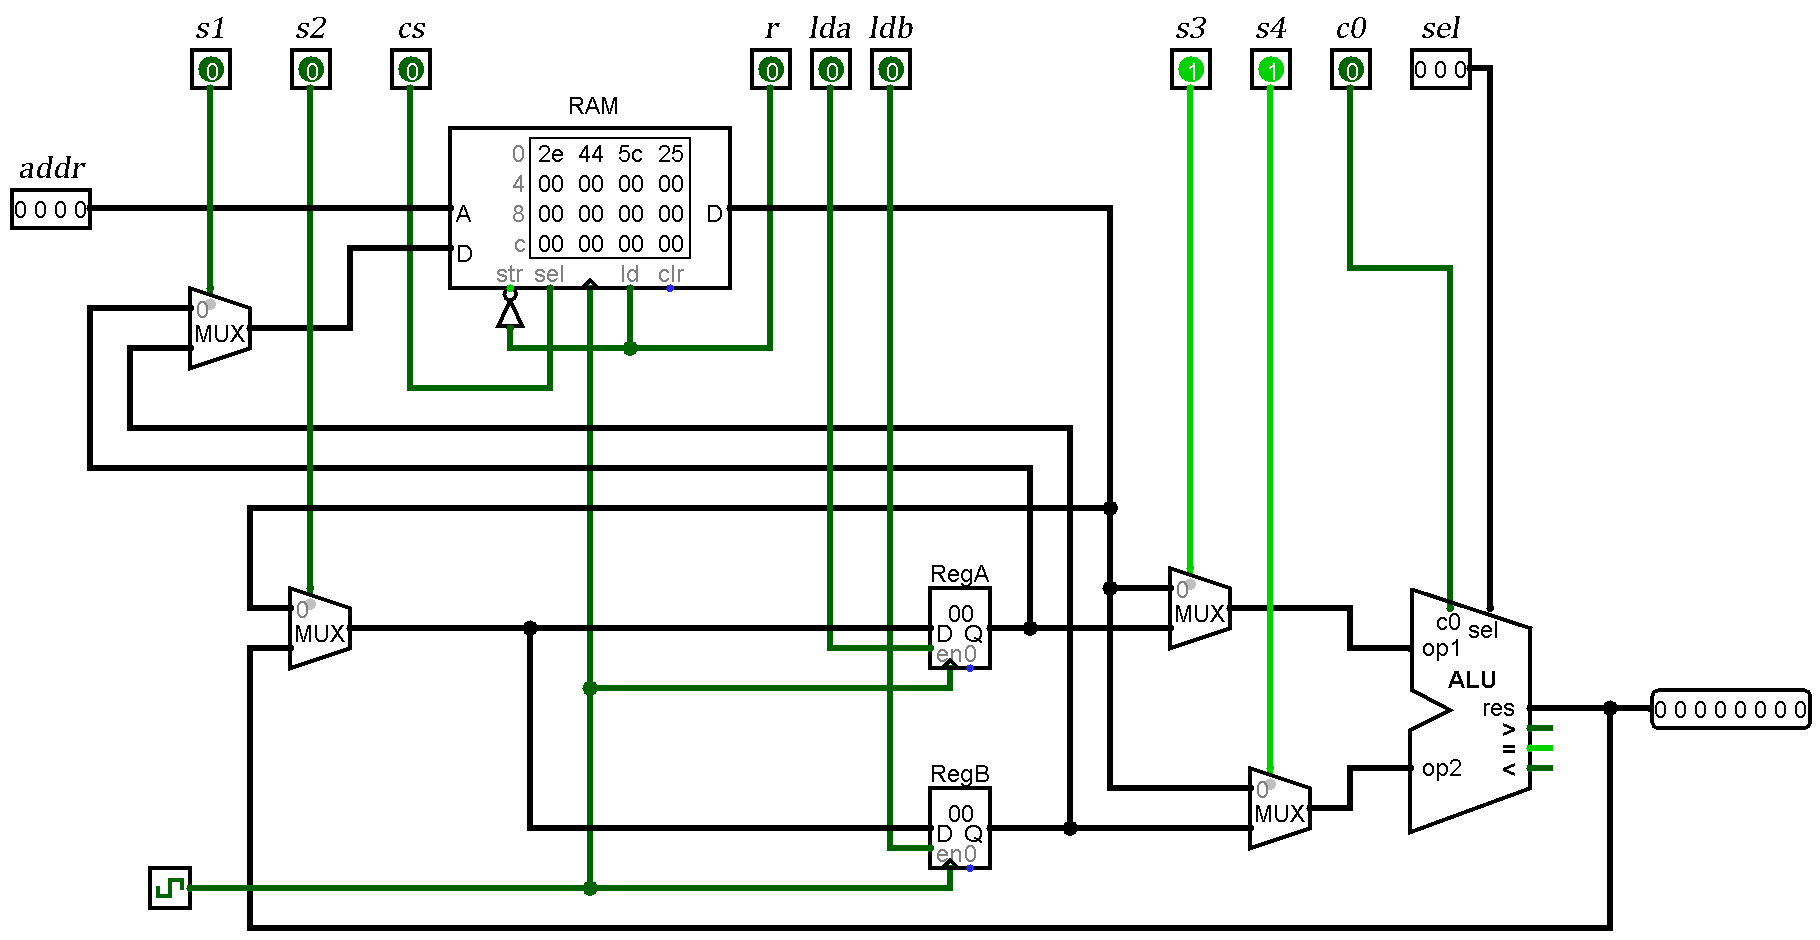
\includegraphics[width=15.5cm]{images/datapath_ex.png}

This datapath contains two 8-bit parallel load registers $A$ and $B$, a $2^4 \times 8$ RAM, and an 8-bit ALU with the function table below (NOTE - this is more or less the ALU described during the combinational logic lecture):

\begin{tabular}{c | l | c | l}
$sel$ & Function & $sel$ & Function \\
\hline
{\tt 0 0 0} & $res = op1 + c0$ & {\tt 1 0 0} & $res = c0$ \\
{\tt 0 0 1} & $res = op1 + op2 + c0$ & {\tt 1 0 1} & $res = op2 + c0$ \\
{\tt 0 1 0} & $res = op1 + \sim op2 + c0$ & {\tt 1 1 0} & $res = \sim op2 + c0$ \\
{\tt 0 1 1} & $res = op1 \land op2$ & {\tt 1 1 1} & $res = op1 \lor op2$ \\
\end{tabular}

For the next four parts of this question, you are to analyze the circuit to determine a sequence of appropriate assignments to every control input of the datapath (including $addr$), so that the final result of the required computation is stored into RAM at the specified address(es).

Some notes and guidelines:

\begin{itemize}
    \item Each 8-bit word in RAM is shown as hexadecimal (e.g. ${\tt2e}_{16} = 46_{10}$). Assume that negative numbers are represented using two's complement.
    \item Carefully study the diagram to observe the flow of 8-bit data values to/from registers and RAM.
    \item If any synchronous device is not involved in one of your intended operations, ensure that the device does not overwrite its contents during the operation (i.e. disable the device using $ld\_$ or $cs$ appropriately).
    \item In most cases, it is better practice to move needed values from RAM into the work registers for computation, and once a work register contains a result (or intermediate result), move it back to RAM unless you can use it again immediately.
    \item You may not overwrite your given initial data values in RAM.
    \item In completing the provided tables, write a 0 or 1 if the control input \textit{must} receive a 0 or 1 for the current operation. If the control input can receive either 0 or 1 without affecting the intended operation, write X (don't care).
    \item In the "Operation" column of the table, use register transfer notation to write a reasonable summary of the general operation.
    \item If testing your mini-program on the provided Logisim file, operations combining RAM retrieval with register storage and ALU \textit{might} require 2 clock cycles (not accurate to real-world microcontrollers, but it's the best Geoff could do in Logisim with the built-in RAM and register devices and this datapath configuration). Make sure your register load control is only active on the second clock cycle.
\end{itemize}

\newpage

  \begin{question}{(a)}[4]
  \item[4] Assume that $RAM\left[0\right]$ contains $46_{10}$, $RAM\left[1\right]$ contains $68_{10}$, $RAM\left[2\right]$ contains $92_{10}$, and $RAM\left[3\right]$ contains $37_{10}$. Other entries are unknown and can be overwritten. Determine a sequence of control input assignments to perform $(46 + 68) \uparrow (92 - 37)$ and store the final result into $RAM\left[15\right]$. The first operation is completed for you as an example.
  {\color{NavyBlue}
  \begin{Questions}
  \begin{tabular}{p{5cm} | c | c | c | c | c | c | c | c | c | c | c}
  Operation & $\, addr \,$ & $\, s_1 \,$ & $\, s_2 \,$ & $\, cs \,$ & $\, r \,$ & $\, lda \,$ & $\, ldb \,$ & $\, s_3 \,$ & $\, s_4 \,$ & $\, c0 \,$ & $\, sel \,$ \\
  \hline
  $RegA \leftarrow RAM\left[0\right]$ & 0000 & X & 0 & 1 & 1 & 1 & 0 & X & X & X & XXX \\
  $RegB \leftarrow RegA + RAM\left[1\right]$ & 0001 & X & 1 & 1 & 1 & 0 & 1 & 1 & 0 & 0 & 001 \\
  $ RAM\left[4\right] \leftarrow RegB$ & 0100 & 1 & X & 1 & 0 & 0 & 0 & X & X & X & XXX \\
  $RegB \leftarrow RAM\left[3\right]$ & 0011 & X & 0 & 1 & 1 & 0 & 1 & X & X & X & XXX \\
  $RegB \leftarrow RAM\left[2\right] + \lnot RegB$ + 1& 0010 & X & 1 & 1 & 1 & 0 & 1 & 0 & 1 & 1 & 010 \\
  $RegB \leftarrow RAM\left[4\right] \land RegB$ & 0100 & X & 1 & 1 & 1 & 0 & 1 & 0 & 1 & X & 011 \\
  $RegB \leftarrow \lnot RegB$ & XXXX & X & 1 & 0 & X & 0 & 1 & X & 1 & 0 & 110 \\
  $ RAM\left[15\right] \leftarrow RegB$ & 1111 & 1 & X & 1 & 0 & 0 & 0 & X & X & X & XXX \\
  \end{tabular}
  \end{Questions}
  }
  \item[4] Assume that $RAM\left[3\right]$ contains $73_{10}$. Other entries are unknown and can be overwritten. Determine a sequence of control input assignments, so that $-70_{10}$ is stored into $RAM\left[15\right]$.
  {\color{NavyBlue}
 \begin{Questions}
  \begin{tabular}{p{4.3cm} | c | c | c | c | c | c | c | c | c | c | c}
  Operation & $\, addr \,$ & $\, s_1 \,$ & $\, s_2 \,$ & $\, cs \,$ & $\, r \,$ & $\, lda \,$ & $\, ldb \,$ & $\, s_3 \,$ & $\, s_4 \,$ & $\, c0 \,$ & $\, sel \,$ \\
  \hline
  $RegA \leftarrow RAM\left[3\right]$ & 0011 & X & 0 & 1 & 1 & 1 & 0 & X & X & X & XXX \\
  $RegB \leftarrow 0 $ & XXXX & X & 1 & 0 & X & 0 & 1 & X & X & 0 & 100 \\
  $RegA \leftarrow RegA + \lnot RegB$ & XXXX & X & 1 & 0 & X & 1 & 0 & 1 & 1 & 0 & 010 \\
  $RegA \leftarrow RegA + \lnot RegB$ & XXXX & X & 1 & 0 & X & 1 & 0 & 1 & 1 & 0 & 010 \\
  $RegB \leftarrow RegA + \lnot RegB$ & XXXX & X & 1 & 0 & X & 0 & 1 & 1 & 1 & 0 & 010 \\
  $RegB \leftarrow \lnot RegB + 1$ & XXXX & X & 1 & 0 & X & 0 & 1 & X & 1 & 1 & 110 \\
  $ RAM\left[15\right] \leftarrow RegB$ & 1111 & 1 & X & 1 & 0 & 0 & 0 & X & X & X & XXX \\
  \end{tabular}
 \end{Questions}
 }
 \item[4] Assume that $RAM\left[0\right]$ contains $16_{10}$, $RAM\left[1\right]$ contains $38_{10}$, and $RAM\left[2\right]$ contains $61_{10}$. Other entries are unknown and can be overwritten. Determine a sequence of control input assignments, so that $(38 + 61) \text{ mod } 16$ is stored into $RAM\left[15\right]$.\\
 {\color{NavyBlue}
 \begin{Questions}
  \begin{tabular}{p{4.7cm} | c | c | c | c | c | c | c | c | c | c | c}
  Operation & $\, addr \,$ & $\, s_1 \,$ & $\, s_2 \,$ & $\, cs \,$ & $\, r \,$ & $\, lda \,$ & $\, ldb \,$ & $\, s_3 \,$ & $\, s_4 \,$ & $\, c0 \,$ & $\, sel \,$ \\
  \hline$RegA \leftarrow RAM\left[2\right]$ & 0010 & X & 0 & 1 & 1 & 1 & 0 & X & X & X & XXX \\
  $RegA \leftarrow RegA + RAM\left[1\right]$ & 0001 & X & 1 & 1 & 1 & 1 & 0 & 1 & 0 & 0 & 001 \\
  $RegB \leftarrow RAM\left[0\right]$ & 0000 & X & 0 & 1 & 1 & 0 & 1 & X & X & X & XXX \\
  $RegA \leftarrow RegA + \lnot RegB$ + 1& XXXX & X & 1 & 0 & X & 1 & 0 & 1 & 1 & 1 & 010 \\
  $RegA \leftarrow RegA + \lnot RegB$ + 1& XXXX & X & 1 & 0 & X & 1 & 0 & 1 & 1 & 1 & 010 \\
  $RegA \leftarrow RegA + \lnot RegB$ + 1& XXXX & X & 1 & 0 & X & 1 & 0 & 1 & 1 & 1 & 010 \\
  $RegA \leftarrow RegA + \lnot RegB$ + 1& XXXX & X & 1 & 0 & X & 1 & 0 & 1 & 1 & 1 & 010 \\
  $RegA \leftarrow RegA + \lnot RegB$ + 1& XXXX & X & 1 & 0 & X & 1 & 0 & 1 & 1 & 1 & 010 \\
  $RegA \leftarrow RegA + \lnot RegB$ + 1& XXXX & X & 1 & 0 & X & 1 & 0 & 1 & 1 & 1 & 010 \\
  $ RAM\left[15\right] \leftarrow RegA$ & 1111 & 0 & X & 1 & 0 & 0 & 0 & X & X & X & XXX \\
    
  \end{tabular}
 \end{Questions}
 }
 \item[4] All entries are unknown and can be overwritten. Store $00_{16}$ into $RAM\left[0\right]$ and $RAM\left[2\right]$, and store ${\tt ff}_{16}$ into $RAM\left[1\right]$ and $RAM\left[3\right]$.\\
 {\color{NavyBlue}
 \begin{Questions}
  \begin{tabular}{p{4.3cm} | c | c | c | c | c | c | c | c | c | c | c}
  Operation & $\, addr \,$ & $\, s_1 \,$ & $\, s_2 \,$ & $\, cs \,$ & $\, r \,$ & $\, lda \,$ & $\, ldb \,$ & $\, s_3 \,$ & $\, s_4 \,$ & $\, c0 \,$ & $\, sel \,$ \\  

  \hline
  $RegB \leftarrow 0 $ & XXXX & X & 1 & 0 & X & 0 & 1 & X & X & 0 & 100 \\
  $ RAM\left[0\right] \leftarrow RegB$ & 0000 & 1 & X & 1 & 0 & 0 & 0 & X & X & X & XXX \\
  $ RAM\left[2\right] \leftarrow RegB$ & 0010 & 1 & X & 1 & 0 & 0 & 0 & X & X & X & XXX \\
  $RegB \leftarrow \lnot RegB $ & XXXX & X & 1 & 0 & X & 0 & 1 & X & 1 & 0 & 110 \\
  $ RAM\left[1\right] \leftarrow RegB$ & 0001 & 1 & X & 1 & 0 & 0 & 0 & X & X & X & XXX \\
  $ RAM\left[3\right] \leftarrow RegB$ & 0011 & 1 & X & 1 & 0 & 0 & 0 & X & X & X & XXX \\
  \end{tabular}
 \end{Questions}
 }
 \vspace{2.0cm}
 
You may have noticed that some of the operations you are asked to do (e.g. NAND), are not directly supported by the ALU. It is the job of the \textbf{compiler} to turn a high-level instruction into a sequence of ALU-supported low-level instructions that produce the required result. Thank you for your effort in this course, good luck with the rest of your studies!

\end{question}


\end{question}

\end{document}





 

